\section{Stima di modelli non lineari nei parametri}
Fin ora abbiamo visto solo come stimare con modelli lineari, quindi nel caso più semplice. Nel caso lineare ci troviamo nella forma:
  \[ Y=\Phi(u)\theta+V \]
ma nel caso non lineare nei parametri, il nostro sistema diventa:
  \[ Y=\Phi(u,\theta)+V \]
I criteri e le ipotesi degli stimatori visti precedentemente rimangono validi, la differenza fondamentale è che non è possibile trovare una forma esplicità dello stimatore (come abbiamo fatto e dimostrato nei casi lineari); ovvero non è possibile trovare un formula per il parametro che minimizza:
\[ J(\theta)=\varepsilon^T(\theta)\varepsilon \]
Per trovare un risultato si ricorre a metodi iterattivi. L'obiettivo degli algoritmi iterattivi è di partire da un punto ed avvicinarsi al minimo della funzione per passi.
\subsubsection{Algoritmo di Gauss -Newton}
\index{Gauss-Newton, algoritmo}
Supponiamo di voler risolvere:
\[ \hat{\theta}=\arg \min_{\theta} J(\theta)=\arg \min_{\theta} \varepsilon^T(\theta)\psi^{-1}\varepsilon(\theta)=\arg \min_{\theta} (Y-\Phi(u,\theta))^{-1}(Y-\Phi(u,\theta)) \]
(la presenza di $\psi$ è casuale, poteva non esserci, dipende dal problema). Definiamo ora con $\theta^k$ l'approssimazione di $\hat{\theta}$ al'iterazione k, e calcoliamo:

  \begin{align*}
    \Phi_\theta^k&={\frac{d\Phi(u,\theta)}{d\theta}}|_{\theta=\theta^k}\\
    \tilde{\theta}^k&=\theta-\theta^k\\
    \widetilde{Y}^k&=Y-\Phi(u,\theta^k) 
  \end{align*}
  
Per lo sviluppo di Taylor (troncata al primo grado) possiamo scrivere:

  \begin{gather*}
    \Phi(u,\theta) \cong \Phi(u,\theta^k) + \Phi_\theta^k(\theta-\theta^k)\\
    \varepsilon(\theta) = Y-\Phi(u,\theta) \cong Y-\Phi(u,\theta^k) - \Phi_\theta^k(\theta-\theta^k)=\widetilde{Y}^k-\Phi_\theta^k\tilde{\theta}^k
  \end{gather*}
  
Ne consegue quindi che:

  \[ J(\theta)\cong J^k(\tilde{\theta}^k)=(\widetilde{Y}^k-\Phi_\theta^k\tilde{\theta}^k)^T\psi^{-1}(\widetilde{Y}^k-\Phi_\theta^k\tilde{\theta}^k) \]
  
Ora la minimizzazione di $J^k(\tilde{\theta}^k)$ è un problema standard, infatti:

  \[ \hat{\tilde{\theta}}^k=((\Phi_\theta^k)^T\psi^{-1}\Phi_\theta^k)^{-1}(\Phi_\theta^k)^T\psi^{-1}\widetilde{Y}^k \]
  
ricordando che $\theta=\theta^k+\tilde{\theta}^k$, è logico che $\theta^{k+1}=\theta^k+\hat{\tilde{\theta}}^k$ e quindi:

  \[ \theta^{k+1}=\theta^k+[((\Phi_\theta^k)^T\psi^{-1}\Phi_\theta^k)^{-1}(\Phi_\theta^k)^T\psi^{-1}\widetilde{Y}^k] \]
  
\paragraph{Osservazione 1} Non c'è alcuna garanzia di convergenza ad una soluzione. Se anche dovesse convergere potrebbe finire in un minimo locale e non nel minimo globale che andiamo cercando. Eseguendo più volte l'algoritmo, se si ottengono valori diversi [FIXME: non si capisce cosa ci sia scritto negli appunti]
%FIXME NON SI CAPISCE COSA C'È SCRITTO NEGLI APPUNTI
\paragraph{Osservazione 2} Potrebbe accadere che $det(((\Phi_\theta^k)^T\psi^{-1}\Phi_\theta^k))\cong 0$ e quindi non è detto che il problema sia identificabile. Per ovviare a ciò si modifica l'algoritmo aggiungendo un parametro $\alpha^k$ che rende il determinante positivo:

  \[ \theta^{k+1}=\theta^k+[((\Phi_\theta^k)^T\psi^{-1}\Phi_\theta^k+\alpha_kI)^{-1}(\Phi_\theta^k)^T\psi^{-1}\widetilde{Y}^k] \]
  
Questa variazione va sotto il nome di Levenberg - Marquardt. La variabile $\alpha^k$ viene posta a zero quando il determinante è già significativamente diverso da zero, altrimenti viene posta ad un valore piccolo. In questo modo il determinante viene positivo e l'algoritmo prosegue nella minimizzazione
\paragraph{Osservazione 3} Convergenza quadratica nell'intorno del minimo:

  \[ \| \theta^{k+1}-\theta^k \|\leq \| \theta^k - \theta^{k-1}\|^2  \]
  
non garantisce la convergenza al minimo globale, quindi spesso si usano algoritmi medi.

\begin{center} \rule{300pt}{1pt} \end{center}
\begin{esempio} % ####################
Cinetica di un farmaco. Il problema è di capire quanto velocemente diminuisce la concentrazione $c(t)$ di farmaco presente nel corpo e quando ripetere la somministrazione:

\begin{figure}[htbp]
  \centering
  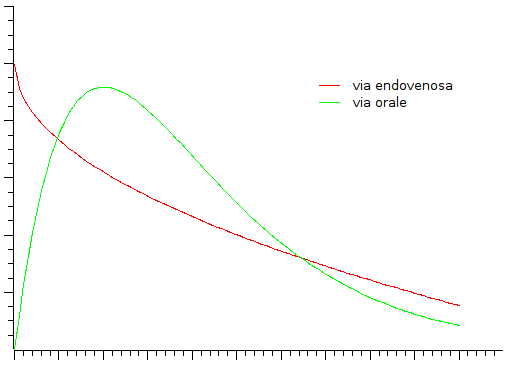
\includegraphics[scale=0.6]{img/cineticafarmaco.png}
  \caption{Cinetica di un farmaco\label{fig:cineticafarmaco}}
\end{figure}

%FIXME dagli appunti online è poco chiaro
[FIXME dagli appunti online è poco chiaro]
\end{esempio}

\begin{esempio} % ####################
Scelta tra due modelli
%FIXME dagli appunti online è poco chiaro
[FIXME dagli appunti online è poco chiaro]
\end{esempio}
\begin{center} \rule{300pt}{1pt} \end{center}
